\chapter{Prototip}
\label{chap:Prototip}

%Introducció
El nostre prototip consisteix en un BMS capaç de balancejar cel·les, controlar la temperatura i la càrrega i descàrrega. Aquests són els principals factors que cal controlar d'una bateria. Cal destacar que el BMS és modular, és a dir, que es poden afegir diferents mòduls per augmentar el nombre de cel·les i per tant el voltatge. D'aquesta manera depenent del nombre de cel·les hi hauran més o menys mòduls i per tant el nombre de bateries que pot controlar és més flexible. A més a més el nostre prototip incorpora un control extern del BMS basat en l'integrat d'Atmel (Arduino) de la placa BMS. Pel nostre prototip només s'ha arribat a plantejar la placa BMS mestre, no s'ha tingut en compte els BMS esclaus ja que no s'ha pogut assolir el projecte fins a l'objectiu plantejat a l'inici.

Avui en dia l'electrònica està molt avançada i és per això que no cal \newline necessàriament dissenyar un BMS des de zero, ja que es proveeixen certes parts, les quals faciliten molt la implementació. Aquests mòduls venen en forma d'integrats i pràcticament s'encarreguen de la part més complexe del que seria un BMS en la seva totalitat. És per això que ens hem basat en un d'aquests integrats per tal d'implementar de forma teòrica un prototip de BMS. 

\section{Selecció de l'integrat per al prototip BMS}
En primera instància, al moment d'indagar sobre possibles integrats per al nostre prototip vam veure un xip de la família Atmel que ens va cridar molt l'atenció. Aquest xip era el ATA6870N. La part bona d'aquest integrat és que ja hi havia un projecte a Internet el qual serviria molt bé com a guia. Aquest projecte proporcionava tant el hardware com el software del BMS i facilitava molt la seva implementació real. Quan vam veure que era viable vam escollir aquest integrat per al prototip. Dos mesos després de feina, quan vam començar a pressupostar el prototip, ja que el disseny ja el teníem, ens vam adonar que aquest integrat es va deixar de fabricar feia uns mesos ja que l'empresa Atmel va tancar. Per tal de no fer servir un integrat que estava fóra del mercat es va haver de redirigir tot el projecte amb l'elecció d'un nou integrat. Aquest integrat és el BQ76pl455a-q1. 

Aquest integrat supera en gran mesura la complexitat i abast de l'integrat d'Atmel. Controla més cel·les, té un disseny més elaborat, permet comunicacions aïllades entre mòduls, entre d'altres aplicacions. La part negativa es que no donen un disseny total d'un BMS ni el software. Per tant la implementació real es complica en gran mesura. Per anomenar d'una forma més còmoda aquest integrat li direm BQ.

\begin{figure}[H]
	\centering
    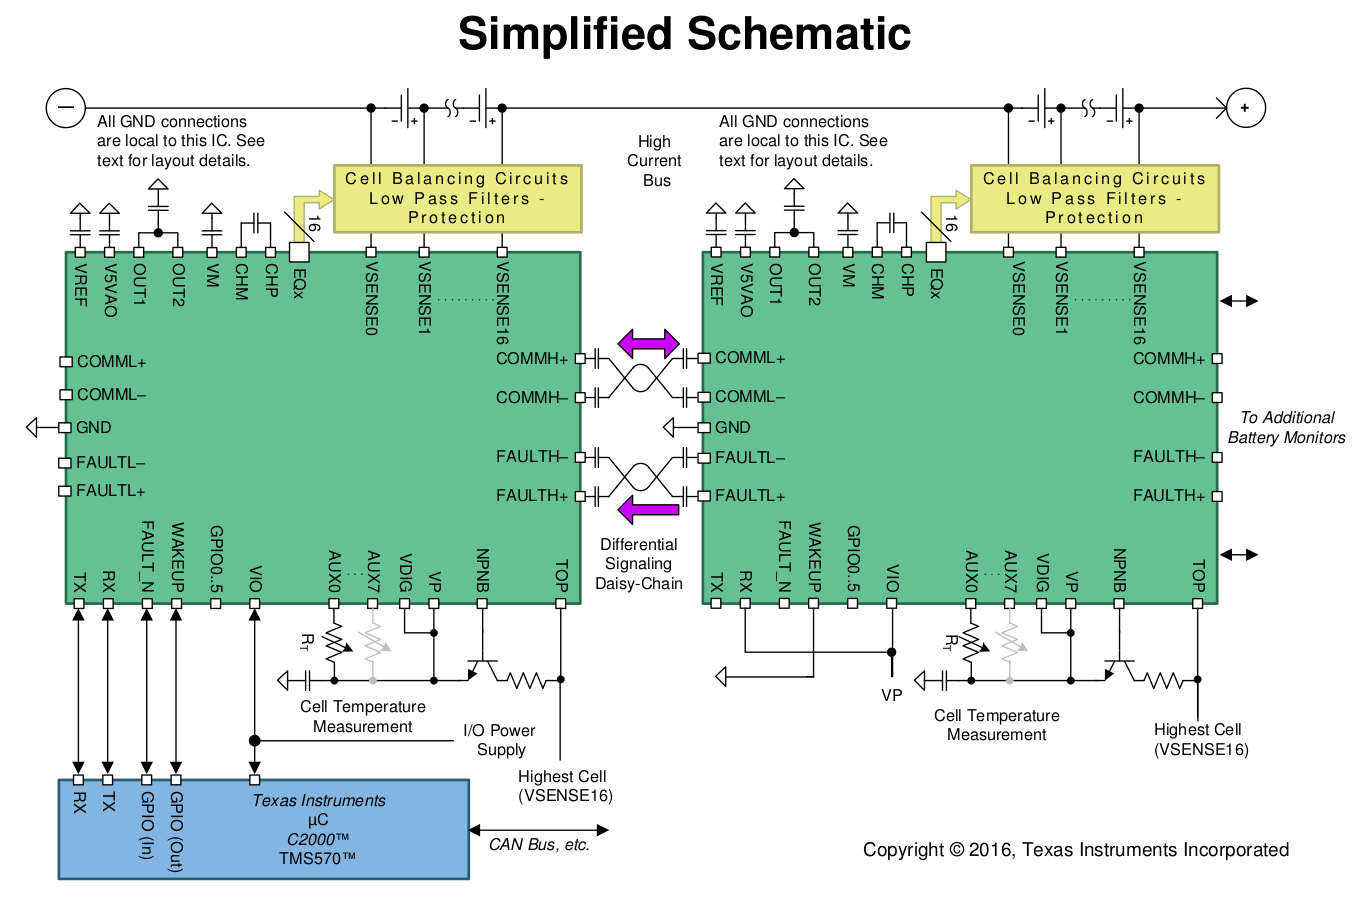
\includegraphics[width=\textwidth, height=10cm] {Prototip/esquematicsimplificat.png}
    \caption{Diagrama simplificat del BQ76pl455a-q1.}
\end{figure}

\section{Coneixent l'integrat BQ76pl455a-q1 }

El BQ és un integrat preparat per a monitorar i protegir fins a 16 cel·les, amb un disseny d'alta confiança per a motors elèctrics. La gran velocitat de l'integrat, la comunicació capacitiva aïllada diferencial i l'alta diversitat de possibles comunicacions ha fet que ens decantéssim per aquest integrat. Lo bo d'aquest integrat es que monitora i detecta un munt de diferents possibles condicions de falla, incloent: sobrevoltatge, sota voltatge, sobre temperatura i falles de comunicació. També té entrades digitals i analògiques per afegir monitoreig addicional i funcionalitats de programació. També incorpora una parada d'emergència en cas de sortir dels rangs de temperatura que s'admeten en una bateria.

Les aplicacions principals d'aquest integrat són per al control de vehicles elèctrics, sistemes de 48V quan només s'utilitza un únic integrat, per emmagatzemament d'energia (UPS) i per a bicicletes elèctriques.

A continuació s'esposarà el funcionament d'aquest integrat per a les diferents funcionalitats que proveeix.

\subsection{Màquina d'estats del BQ}

L'integrat escollit per aquest projecte té molts estats interns que succeeixen en la seva electrònica, però a grans trets estan diferenciat en tres estats: Shutdown, Idle i Wake up. L'estat de Shutdown seria quan la bateria no estigués connectada al BMS i per tant, no estigués rebent corrent el microcontrolador. També podria ser que es forcés una parada des del microcontrolador. És l'estat de parat. L'estat Idle és l'estat de funcionament i és on tot està funcionant, tant el balanceig, el monitoreig, processament de dades... En definitiva, tot el que envolta les funcions d'un BMS. L'estat de Wake up consisteix en el moment en el que el BQ passa d'estar de Shutdown a estat Idle. Es converteix en un estat ja que el seu procés és bastant complexe. De no ser així estaríem parlant de la màquina d'estats més simple que hi pot haver, que funciona o no funciona, encara que el BQ presenta algunes característiques especials quan està en mode Shutdown.

\subsubsection{Estat de funcionament (IDLE state)}
No s'entrarà en detall ja que és quan el BQ no es troba en cap dels altres dos estats. Simplement és quan l'integrat està en funcionament, és a dir, està realitzant la funció de control en un BMS. Sempre i quan surti de la funció de BMS sobre una bateria es trobarà en els altres dos estats. Al llarg d'aquest capítol es parlarà sobretot del funcionament del BQ com a BMS i per tant, estarem parlant tota l'estona de l'IDLE state.

\subsubsection{Estat d'encesa (Wake up state)}
L'estat d'encesa pot ser ocasionat per dos únics factors. En primer lloc l'integrat disposa d'un pin anomenat \textit{WAKEUP} que si es posa en estat alt quan el BQ està apagat el posa en estat d'encesa. Aquest pin només està pensat per a la placa mestre del BMS, la qual estaria connectada a un microcontrolador. El microcontrolador seria l'encarregat de posar en marxa l'integrat posant a nivell alt el pin de \textit{WAKEUP}. Aquest pin només té sentit per als BMS mestres ja que en cas de que hi hagin connectats mòduls esclaus, aquests seran activats mitjançant les comunicacions. 

En el cas en el que hi hagi un BMS mestre i diferents mòduls esclaus en el moment que s'apliqui un senyal que provoqui l'estat d'encesa quan l'integrat està apagat, cal que torni a nivell baix per a que l'integrat pugui tornar a l'estat de parada. En aquest moment, el BQ transmetrà el senyal d'encesa pels seus pins de communicació al següent mòdul esclau, on els pins de communicació el rebran i rebotaran cap al següent mòdul.

El pin de \textit{WAKEUP} usualment es troba a nivell baix. Si aquest pin es posa a nivell alt i l'equip ja havia estat avisat per parar-se, immediatament es tornarà a encendre i posar en estat de funcionament. Per evitar problemes, aquest pin no pot estar mai flotant, sempre cal que estigui definit a nivell alt o baix. Mentre l'integrat es troba en estat apagat els pins de communicació que connecten amb el mòdul adjacent més proper a la placa mestre estan escoltant per a si reben un senyal d'encesa. 

Si el pin de \textit{WAKEUP} es posa a nivell alt quan l'integrat està en l'estat de funcionament es provoca un reset i l'integrat torna a començar per l'estat de Wakeup.

\subsubsection{Estat de parada (Shutdown)}

L'estat de parada és l'estat de potència més baix disponible per al BQ. En aquest estat el BMS talla la potència de la bateria, deshabilita el monitoreig per a la majoria de blocs interns, inclosos els de control. Típicament, l'estat de parada són per a períodes llargs d'inactivitat quan la bateria no estigui sent carregada o descarregada. La part que ha de rebre el senyal per a que el BMS es posi en funcionament és a través del pin de \textit{WAKEUP} o per les comunicacions entre plaques mestre i esclau, ja que les comunicacions es queden en mode d'escolta en l'estat de parada. 

Per entrar en l'estat de parada, s'ha de deixar d'alimentar els pins que alimenten l'integrat; el VP i el VDIG. El pin VIO pot romandre alimentat en l'estat de parada. Els pins VP i VDIG han d'estar totalment desconnectats ja que sinó provocarien una potència negativa. El pin de \textit{WAKEUP} ha d'estar en tot moment a nivell baix per a què no tregui a l'integrat de l'estat de parada. 

Totes les condicions que poden provocar un estat de parada queden resumides en els següents punts:

\begin{itemize}
    \item A través del microcontrolador s'envia un ordre de \textit{SHUTDOWN}.
    \item Timeout ocasionat a les comunicacions.
    \item El voltatge VDIG té valors inferiors al seu llindar mínim.
    \item Un dels sensors interns de temperatura detecta un valor fora dels llindars.
    \item Detecció de falla en els controls de l'integrat.
\end{itemize}

En el nostre cas com que tot el disseny estarà implementat en una mateixa placa, i el pistejat d'aquesta serà fixa, no podrem aprofitar l'ús del VIO en el nostre BMS per alimentar al microcontrolador, ja que s'alimenta de la pròpia bateria que en estat de SHUTDOWN el microcontrolador la talla. 

\subsection{Voltatges de funcionament del BQ}

El BQ té la peculiaritat de que s'alimenta fent ús de la pròpia bateria que gestiona, si les cel·les no estan connectades el microcontrolador no funciona. Un integrat sol treballar a voltatges petits d'un valor d'entre 5 i 7 volts per norma general. Si s'alimenta de la pròpia bateria estem parlant de fins a valors d'uns 60V. Cal d'una electrònica externa per tal de convertir aquests 60V en un voltatge òptim per al microcontrolador. 

\begin{figure}[H]
	\centering
    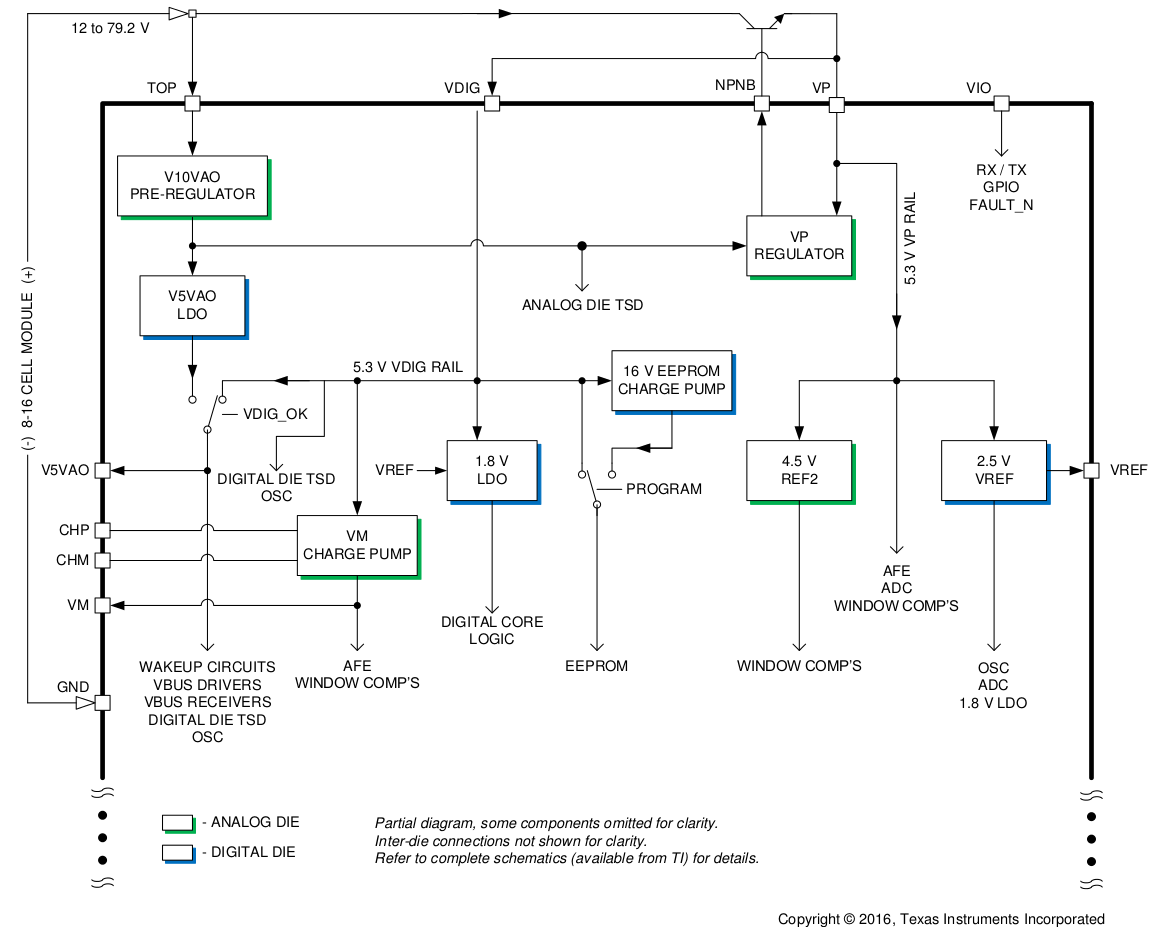
\includegraphics[width=\textwidth, height=10cm] {Prototip/diagramavoltaje.png}
    \caption{Diagrama complert de voltatge.}
\end{figure}

\subsubsection{Alimentació de l'integrat (VP i TOP)}
Com s'acaba de comentar els integrats treballen a uns valors electrònics molt inferiors al voltatge de la bateria que s'està tractant en aquest prototip. Els límits de l'alimentació d'entrada es troben entre -0.3 i 5.5V. Cal reduir doncs aquest voltatge elevat en uns valors vàlids per a l'integrat. El pin d'entrada d'alimentació és el VP. 

Per a tractar aquest voltatge el fabricant recomana l'ús d'un transistor NPN de potència per generar una nominal de 5.3V, que és el voltatge de funcionament òptim per a l'integrat. El tret del transistor es realitza internament mitjançant el pin NPNB. En el moment que la bateria es connecta, internament el pin NPNB s'activa i dispara el transistor per alimentar l'integrat. Quan arriba el senyal al transistor ja ve filtrat per dos filtres pas-baix per tal de reduir al màxim el soroll. És molt important controlar el corrent en aquest punt ja que la potència ve directa de les cel·les on està connectada. El corrent és de de la cel·la més alta fins a la cel·la més baixa del muntatge de cel·les. La cel·la més alta de la bateria es connecta també al pin TOP. Aquesta connexió es realitza amb un filtre pas-baix per evitar efectes de soroll, ja que les bateries en generen molt. El filtre pas-baix sol tenir una constant de temps similar a les entrades VSENSE.

El pin TOP també s'utilitza per a l'alimentació de l'integrat i com a mesura total de la bateria, un cop filtrat el senyal. Aquesta mesura és la que indica per medi del hardware l'activació del pin NPNB.

\subsubsection{Alimentació interna de l'integrat (VIO i VDIG)}
Del col·lector del transistor NPN de potència emprat per a l'alimentació de l'integrat, també se n'aprofita una part el pin VIO. Aquest pin s'encarrega d'alimentar la part de l'integrat encarregada de les comunicacions amb un microcontrolador. En concret dóna l'alimentació als pins de GPIO, als de communicació Serial (RX/TX) i al pin FAULTN. A més es pot emprar directament el voltatge de sortida del pin VIO per alimentar un microcontrolador. S'emprarà aquesta tècnica per alimentar el micro del nostre prototip i aprofitar ja els 5V filtrats que ens proporciona. Aquest pin pot no estar connectat, encara que es recomana en tots els casos que ho estigui, ja que cal d'un control extern que gestioni el BMS. 

A més a més no només s'aprofita una part del voltatge que entra a VP per a VIO, sinó que al disseny entra un tercer pin que és el VDIG. Aquest pin és l'encarregat de gestionar el voltatge per als components interns de l'integrat encarregats de realitzar els càlculs. Estem parlant dels ADCs que s'impliquen en els càlculs i lectures dels senyals per al correcte funcionament del BMS. El voltatge entrant per VDIG és regulat fins a 1.8 volts, voltatge al qual treballen els ADCs. El pin VDIG ha d'estar alimentat per a que l'integrat funcioni.

\begin{figure}[H]
	\centering
    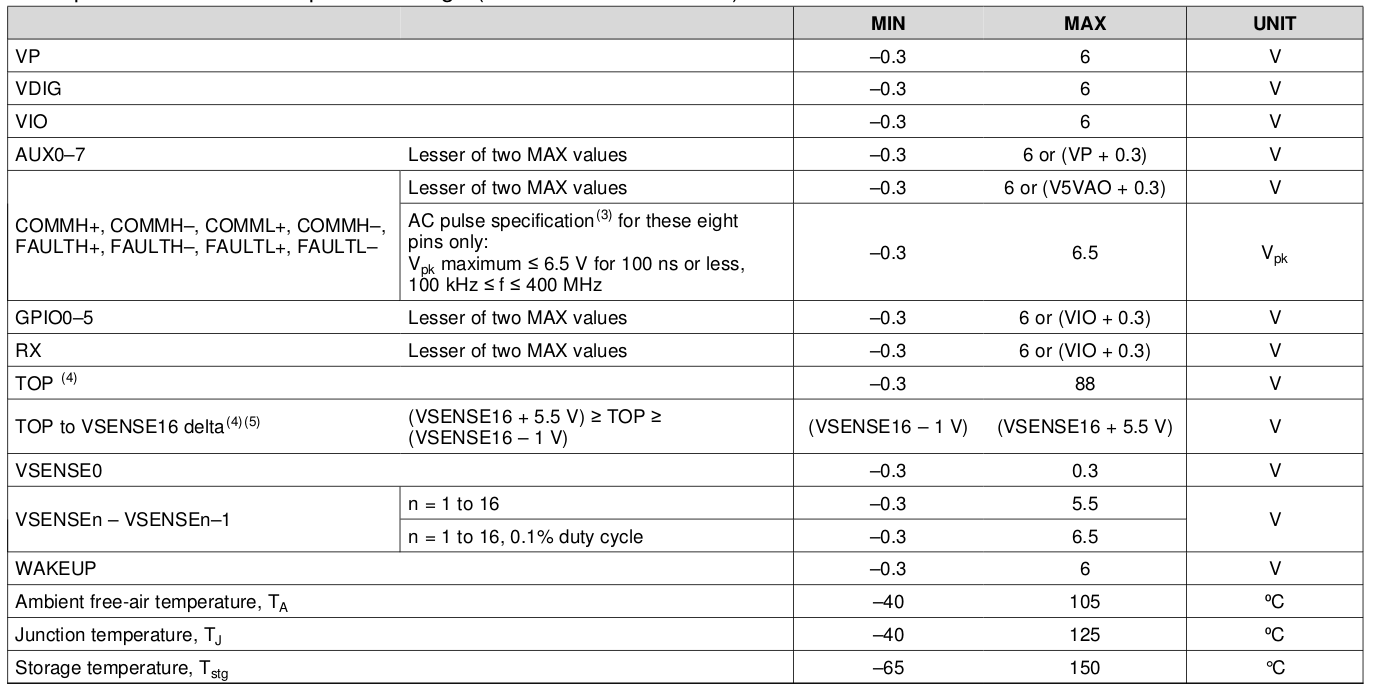
\includegraphics[width=\textwidth, height=8cm] {Prototip/nivelesvoltaje.png}
    \caption{Voltatges de funcionament del BQ76pl455a-q1.}
\end{figure}

\subsection{Balanceig de les cel·les}

Com s'ha anat comentant al llarg del projecte, el balanceig de cel·les és una de les tasques més importants que ha d'implementar un BMS. En termes simples ha de poder mesurar els voltatges de la cel·les i aplicar l'acció pertinent per a que estiguin balancejades en tot moment. Les lectures de les cel·les del nostre prototip es realitzen mitjançant el pin VSENSE (pin on es connecta el pol positiu d'una cel·la), aquest pint té un rang entre 1V i 4,95V. Aquesta lectura indica al microcontrolador el voltatge de cada cel·la i depenent d'aquest, part d'aquest voltatge que està circulant per la cel·la es dissiparà a través del pin EQ i el circuit de dissipació associat per tal d'igualar les capacitats de totes les cel·les. Cal afegir que un cop el voltatge entra al microcontrolador primerament és comparat en uns operacionals que ja per hardware indiquen si s'està detectant un sobrevoltatge o un sotavoltatge. En el moment que un d'aquests operacionals detecta un sobre o sotavoltatge, el microcontrolador ho processa detectant un estat de FAULT, pausant el sistema per evitar riscs sobre altres cel·les o el propi microcontrolador i avisant al microcontrolador d'un estat de FAULT. 
L'adquisició dels valors de voltatge de les cel·les es realitzen en el AFE (Analog Front End). El front-end és doncs on es monitoren fins a 16 cel·les. La programació del BQ es pot configurar per tal que monitori tot, un grup, o les cel·les connectades. El mostreig comença des de la cel·la més alta seleccionada i acaba amb la més baixa seleccionada. Durant la mesura, l'AFE tria la cel·la adreçada per un bloc lògic i el canvi de nivell del voltatge de cel·la detectant un guany d'1 fins el pin OUT1 referenciat a terra. La sortida analògica de l'AFE es connecta a OUT1 a través d'una resistència interna. Externament es connecta al pin OUT2 que és on està connectat l'ADC. Això es fa per aïllar internament la part que gestiona les cel·les amb la part que realitza els càlculs, evitant qualsevol tipus de soroll. En aquesta connexió externa entre l'AFE i l'ADC, el requeriment és posar un filtre RC extern per reduir el soroll a l'ample de banda.

 El BQ proporciona tant balanceig actiu com balanceig passiu, encara que és necessita un petit mòdul addicional per aplicar el balanceig actiu. A més a més el microcontrolador permet el balanceig passiu amb una connexió directa. També és la solució econòmica i per tant tots aquests factors han fet escollir aquest tipus de balanceig. 
 
 El balanceig passiu consisteix en dissipar energia a través de resistències de potències, les quals retenen part del corrent i ho transformen en energia calorífica. Cal tenir en compte quina és la potència que es vol dissipar per tal de fer servir una resistència o un altra. En el nostre cas la dissipació externa podrà ser de fins a 1W. El propi microcontrolador ja porta a l'entrada dels diferents VSENSEn una resistència que ja fa una primera limitació de voltatge.
 
 El BQ implementa doncs el balanceig de les cel·les a través dels pins de EQ1..EQ16. S'utilitzen 16 drivers de control, els quals el fabricant no explica el seu funcionament. Les configuracions de funcions disponibles del balanceig són de l'estil de comandes ON o OFF o específiques per a córrer en un temps específic. L'integrat també disposa d'un registre que habilita o deshabilita el balanceig. Aquest registre pot ser modificat per nosaltres per tal d'activar o desactivar el balanceig. Quan succeeix un problema aquest registre s'automodifica parant el balanceig i evitant possibles errors al BMS. A més l'integrat s'apodera de la sortida EQ de la cel·la i el connecta internament al VSENSE de la cel·la inferior reduint el balanceig de corrent a 0.

\subsection{Control de la temperatura}

La forma en la que aquest integrat controla la temperatura és molt bona. Disposa per defecte un sistema de control de temperatura intern, composat per dos sensors de temperatura connectats directament als ADCs, un per la zona de l'integrat que tracta les cel·les i l'altre per a la pròpia electrònica de control de l'integrat. Aquests sensors mostren la temperatura de forma automàtica al control, el control després té en compte aquests valors per si ha de forçar una parada o reduir el voltatge de les cel·les. El propi integrat ja porta incorporada una protecció per defecte molt bona, ja que es troben a dins de l'integrat. Aquests sensors estan totalment implementats pel fabricant i no cal de cap mena de configuració ja que es basen en les temperatures de funcionament dels components de l'integrat. 

\begin{figure}[H]
	\centering
    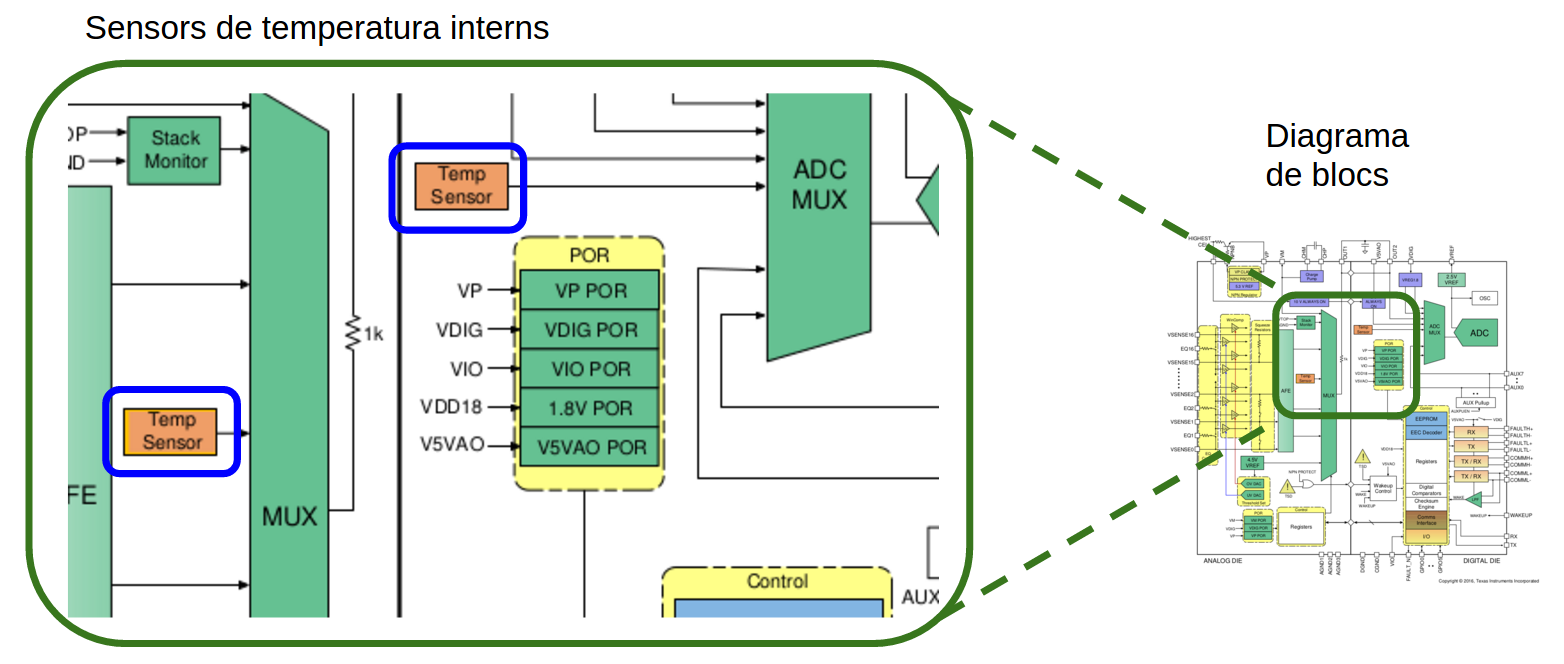
\includegraphics[width=\textwidth, height=7cm] {Prototip/sensorestemperaturainternos.png}
    \caption{Sensors de temperatura interns del BQ76pl455a-q1.}
\end{figure}

A part, el BQ disposa de fins a 8 entrades analògiques de 14 bits (AUX0..AUX7), amb un rang de 0 a 3V per a AUX0 i AUX1, i un rang de 0 a 5V per a la resta d'entrades. Aquests sensors es poden acotar mitjançant uns registres llindars, els quals permeten afinar molt més els rangs. L'ús més comú per aquestes entrades és mitjançant l'ús de termistors. Un termistor és un sensor de temperatura per resistència. El seu funcionament es basa en la variació de la resistivitat que presenta un semiconductor amb la temperatura. Bàsicament es pot mesurar la temperatura a través de termistors.

L'integrat per sí mateix, no té cap mena de control sobre aquests pins AUXn, és a dir que no és capaç de processar les temperatures mostrades per aquests. L'únic que realitza el control és l'enviament d'aquests valors a un microcontrolador. És el microcontrolador qui ha de processar les dades i donar ordre sobre el control. Per defecte, quan s'inicialitza l'integrat comença un comptador cada 1 segon que mostreja els sensors de temperatura, temps més que suficient per a veure l'estat d'una cel·la, ja que no varien tan ràpidament com veure la diferència en 1 segon. 

\subsection{Comunicació entre mòduls BQ}

Per aplicacions on es requereixi múltiples mòduls BQ (un mestre i la resta esclaus), l'integrat proveeix d'un bus de comunicació diferencial que permet al mòdul mestre controlar fins a 16 dispositius, únicament utilitzant una interfície UART. La connexió es realitza en forma de cadena, és a dir, si el mestre és el mòdul 1, els següents mòduls aniran connectats al mòdul adjacent n+1. 

En la configuració en pila, el procés normal de comunicació vindria a ser el següent: 
Primerament el microcontrolador envia una comanda mitjançant el Serial de l'integrat. Un cop el BQ mestre rep les dades, el control genera una communicació que és enviada a través dels diferents mòduls esclau emprant un protocol diferencial de comunicació privatiu del fabricant a través dels pins COMMH+/- i COMML+/-.

Cada equip de la cadena amortigua el senyal. El senyal no es sincronitza o es filtra, passa a través de la cadena i tots els mòduls veuen tota la informació del bus independentment de l'integrat objectiu del senyal. Els paquets arriben a l'ADC de cada un dels integrats i valida el paquet mirant l'adreça objectiu, el contingut del missatge i el CRC. 

\begin{figure}[H]
	\centering
    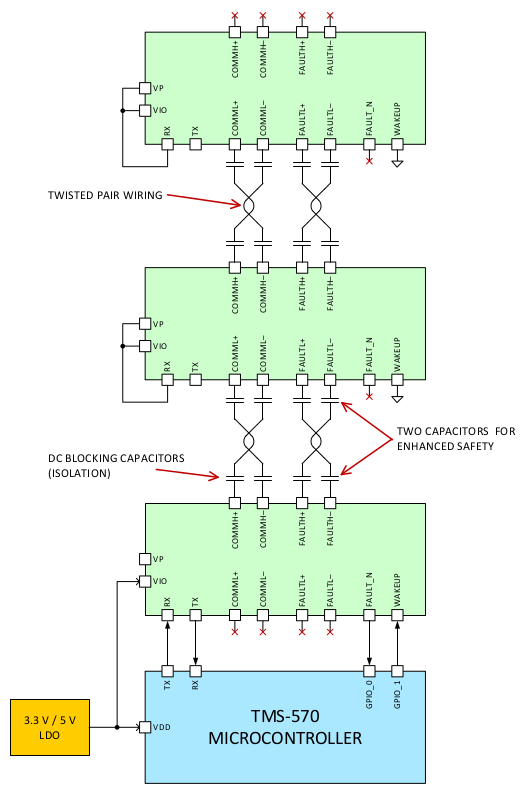
\includegraphics[width=10cm, height=16cm] {Prototip/diagramacomunicacion.png}
    \caption{Connexió entre mòduls BQ76pl455a-q1.}
\end{figure}

\newpage 

En funció del disseny del BMS la communicació entre plaques necessita un disseny o un altre. En el cas que més d'un integrat es trobi en la mateixa PCB no cal un aïllament per a les comunicacions. En canvi, si es troben en PCBs diferents, és obligatori fer ús de components d'aïllament. Quan estan a la mateixa PCB, aquest seria el disseny recomanat pel fabricant:

\begin{figure}[H]
	\centering
    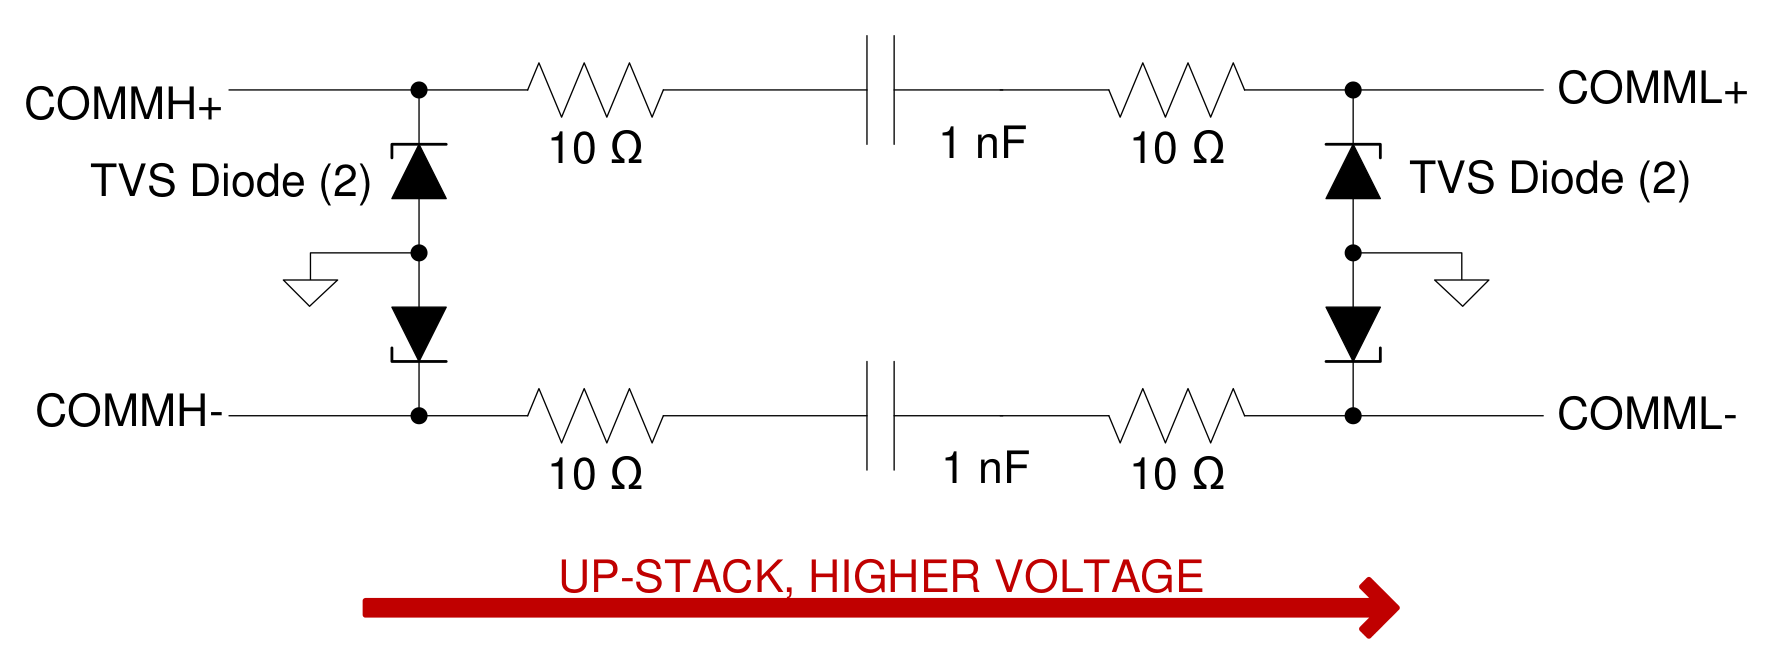
\includegraphics[width=12cm, height=5cm] {Prototip/esquemasamepcb.png}
    \caption{Circuit de connexió entre mòduls BQ a la mateixa PCB.}
\end{figure}

En canvi si els mòduls es troben allotjats en diferents PCBs, el disseny que s'empraria seria el següent:

\begin{figure}[H]
	\centering
    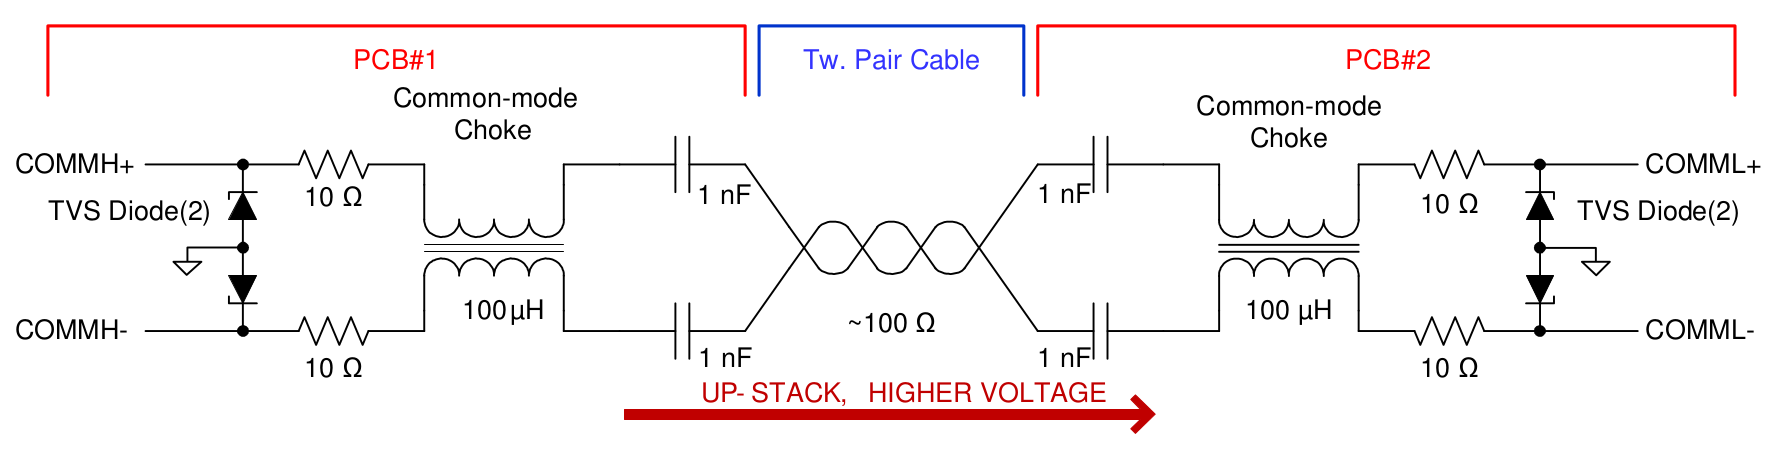
\includegraphics[width=12cm, height=5cm] {Prototip/esquemadifpcb.png}
    \caption{Circuit de connexió entre mòduls BQ en diferents PCB.}
\end{figure}

En el nostre cas ens hem basat en el segon disseny, ja que només tenim pensat posar un mòdul per PCB, on cada un d'aquests integrats controlaria fins a 16 cel·les. En aquest segon disseny l'aïllament es  realitza mitjançant un transformador i condensadors i resistències per a controlar el senyal.

\subsection{Comunicació serial amb el microcontrolador}

El protocol que empra aquest integrat per a la communicació el realitza mitjançant l'UART. Aquest mètode disposa de dos pins de comunicació, un per rebre (RX) i l'altre per enviar (TX). A través d'aquests pins serà per on el microcontrolador enviarà les ordres per a configurar l'integrat d'una manera concreta. 

\subsubsection{UART}
L'UART segueix el protocol estàndard serial 8-N-1, on s'envia la informació com: un bit de START, seguit dels 8 bits d'informació que es necessiten i terminant amb un bit de STOP. La data rebuda per l'integrat està sobre mostrejada per 16 cops per millorar la fiabilitat de la comunicació.

L'integrat permet que es configurin les comunicacions per a esperar un cert temps després de que s'hagi enviat l'últim bit de recepció per començar a transmetre. El protocol és half-duplex. Això vol dir que només pot estar realitzant-se una acció (entre enviar o rebre) a la vegada. Si està enviant dades pel pin TX ignora totalment el pin RX. Per evitar col·lisions és important que el microcontrolador de control estigui correctament programat i esperi a rebre totes les dades enviades per l'integrat. D'haver-hi alguna col·lisió i les comunicacions deixessin de funcionar el microcontrolador hauria d'enviar un reset de la comunicació. El baud rate del canal de comunicacions del BQ permet rangs que arriben al voltant d'1M. L'integrat també permet controlar uns registres que permeten marcar dos temps de timeout si no arriba cap paquet vàlid.  

\subsubsection{GPIO}
Hi ha 6 pins de GPIO al BQ. Poden ser programats com a entrades o com a sortides. Cada GPIO posseeix una resistència interna de pull-up o pull-down per mantenir el pin en tot moment en un estat conegut. Mitjançant la configuració de registres aquests pins es configuren per a ser connectats a la resistència de pull-up o la de pull-down. 

El pin de GPIO permet també enviar un senyal de FAULT. Normalment aquesta acció es realitzada pel pin de FAULTN, però es pot programar per a que els pins de GPIO també l'enviïn. 

\subsubsection{FAULTN}
El pin FAULTN està pensat per a enviar al microcontrolador un estat de fallida per part de l'integrat. En el moment que l'integrat detecta un signe de FAULT, aquest l'envia en forma de pols pel pin FAULTN per avisar al microcontrolador. 

\subsubsection{WAKEUP}
El pin de WAKEUP s'utilitza per encendre el BMS des del microcontrolador. Per a encendre aquest integrat és necessari que aquest pin rebi un senyal de 5V.  A més a més, si l'integrat ja es troba en estat IDLE i el pin de WAKEUP és posa a nivell alt, l'integrat realitzarà un reset.

\subsection{Atmega2560 com a microcontrolador de control}
El prototip es controlarà mitjançant l'integrat de l'Arduino Mega 2560. Donat que aquest tipus de tecnologia s'ha donat al llarg de la carrera, és molt més fàcil d'implementar i programar que no pas un integrat que no coneixem pas. La idea d'aquest control resideix en el fet de que primerament aquest prototip necessitarà d'un seguit de tests els quals validaran el seu funcionament. El fet de tenir un microcontrolador programable ja a la PCB del BMS suposa l'aplicació directe d'aquest, és a dir, cada cop que es vulguin fer canvis en paràmetres el microcontrolador podrà fer-ho directament. A més, com ja s'ha comentat al llarg del projecte, la implementació del BMS ha estat molt més complicada del que primerament ens semblava. És per això que els esquemàtics encara necessiten retocs per tal d'afegir per exemple vies les quals ens serveixin futurament per testejar el BMS. Per la nostra part el que s'ha volgut fer és únicament la implementació del que seria la circuiteria real del BMS. 

\subsection{Diagrama de blocs i disseny exterior}

\subsubsection{Diagrama de blocs}
\begin{figure}[H]
	\centering
    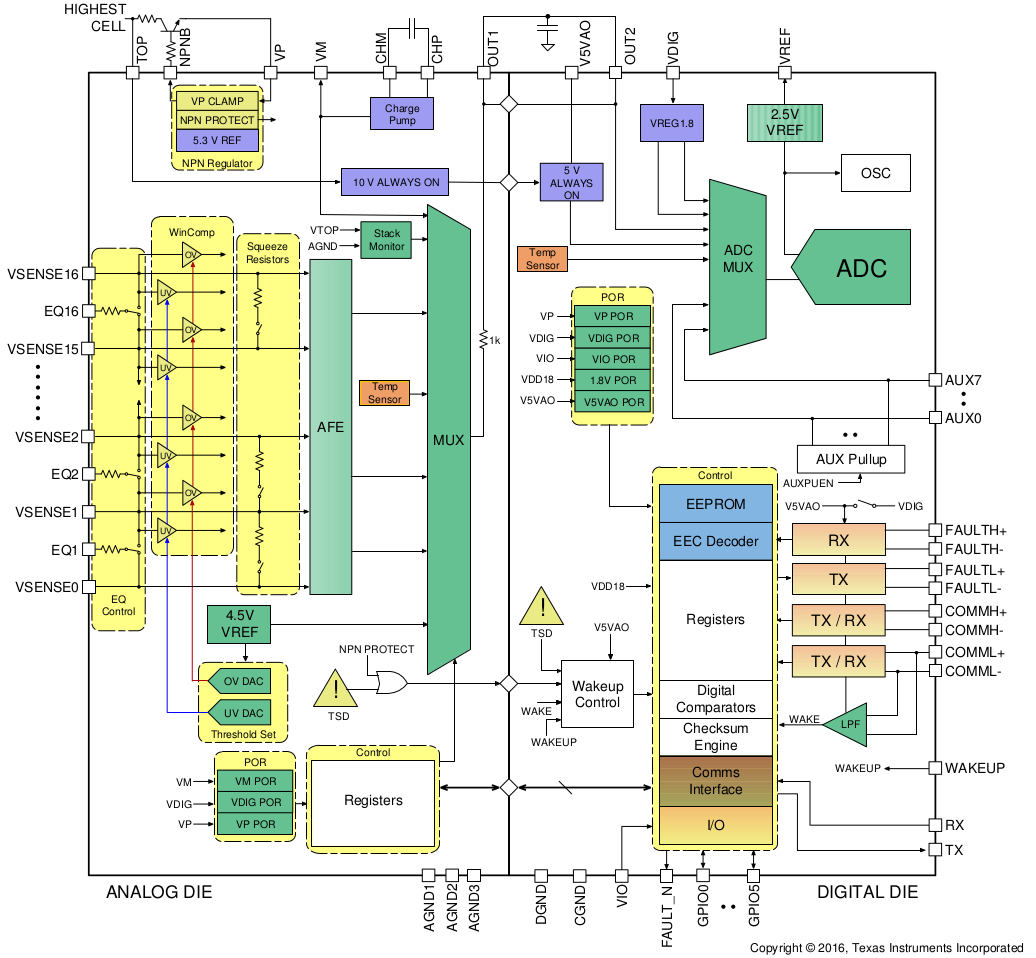
\includegraphics[width=\textwidth, height=14cm] {Prototip/diagramablocs.png}
    \caption{Diagrama de blocs del BQ76pl455a-q1}
\end{figure}

\subsubsection{Disseny exterior}
\begin{figure}[H]
	\centering
    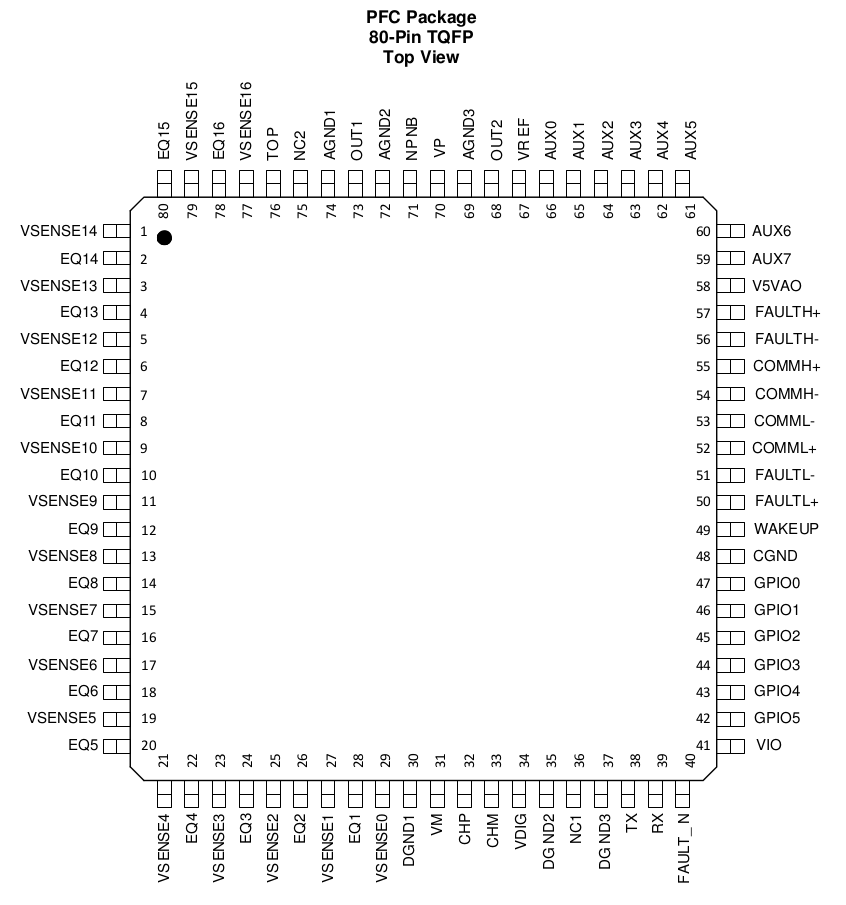
\includegraphics[width=\textwidth, height=14cm] {Prototip/layout.png}
    \caption{Disseny exterior i pins del BQ76pl455a-q1}
\end{figure}

\section{Esquemàtics}

En aquest apartat es mostrarà de forma desglossada els esquemàtics que implementen de forma teòrica el BMS basat en l'integrat BQ76pl455a-q1.

\subsection{Alimentació de l'integrat}
En primer lloc l'alimentació del BQ es realitza per medi del propi corrent de les bateries. Aquest integrat funciona a un rang de 5V mentre que la bateria funciona a uns 60V. L'esquema que es mostra a la figura indica el seu disseny per a passar aquests 60V als 5V. 

\begin{figure}[H]
	\centering
    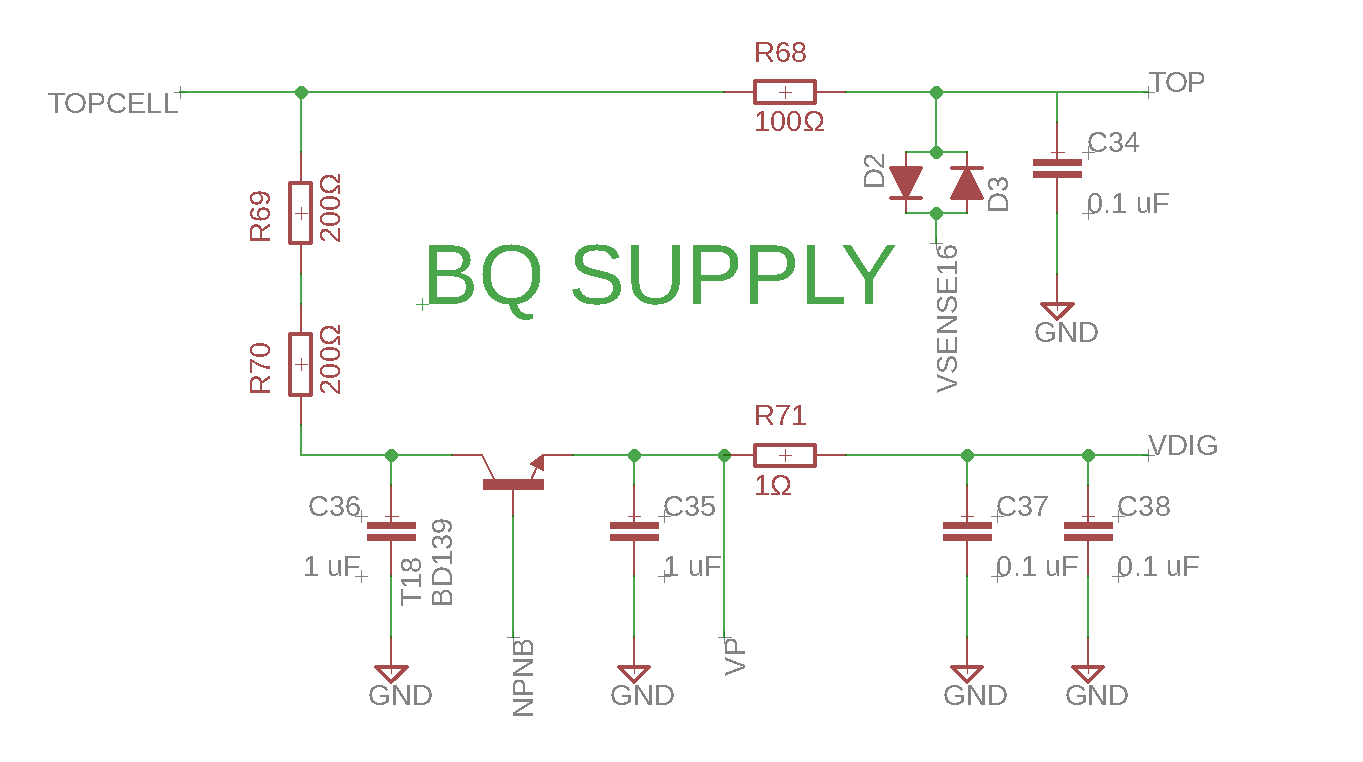
\includegraphics[width=\textwidth, height=8cm] {Prototip/schsupply.png}
    \caption{Alimentació de l'integrat BQ76pl455a-q1.}
\end{figure}

Primerament l'entrada que ve de la bateria ja té un filtrat del soroll \newline mitjançant el doble díode invertit i un filtre RC. Aquí ja el voltatge entra al microcontrolador pel pin TOP. La funció principal d'aquest pin consisteix en fer la lectura total de la bateria. El corrent és novament filtrat fins que arriba al transistor NPNB. Aquest transistor força que l'entrada d'alimentació al pin VP es realitzi a un voltatge de 5V. El col·lector del transistor porta conjuntament amb ell un condensador per evitar canvis bruscs de voltatge. El senyal és novament filtrat i ja entra al pin d'alimentació principal del BQ. El pin VP. A més el senyal és novament filtrat per arribar al pin d'alimentació VDIG, el qual s'encarrega d'alimentar tota la circuiteria dels conversors analògic-digital que incorpora el BQ. D'aquesta manera s'assegura que arriben voltatges de 5V totalment filtrats per evitar tots els problemes que suposa el soroll al corrent.

\subsection{Anivellació de cel·les}

En la següent figura es mostrarà com s'ha implementat l'anivellació de cel·les. Aquí ens hem basat totalment en les especificacions del fabricant ja que es desconeix com l'integrat realitza els algorismes de balanceig. Per VSENSEn entrarà el positiu de la bateria a l'integrat, on és recollirà el voltatge analitzat per l'AFE i enviat al control. El control enviarà aquesta energia a dissipar pel pin EQn. 

Cal destacar que el negatiu de les bateries és diferent al negatiu de tot el BMS, encara que el negatiu també es connecti al BMS.

\begin{figure}[H]
	\centering
    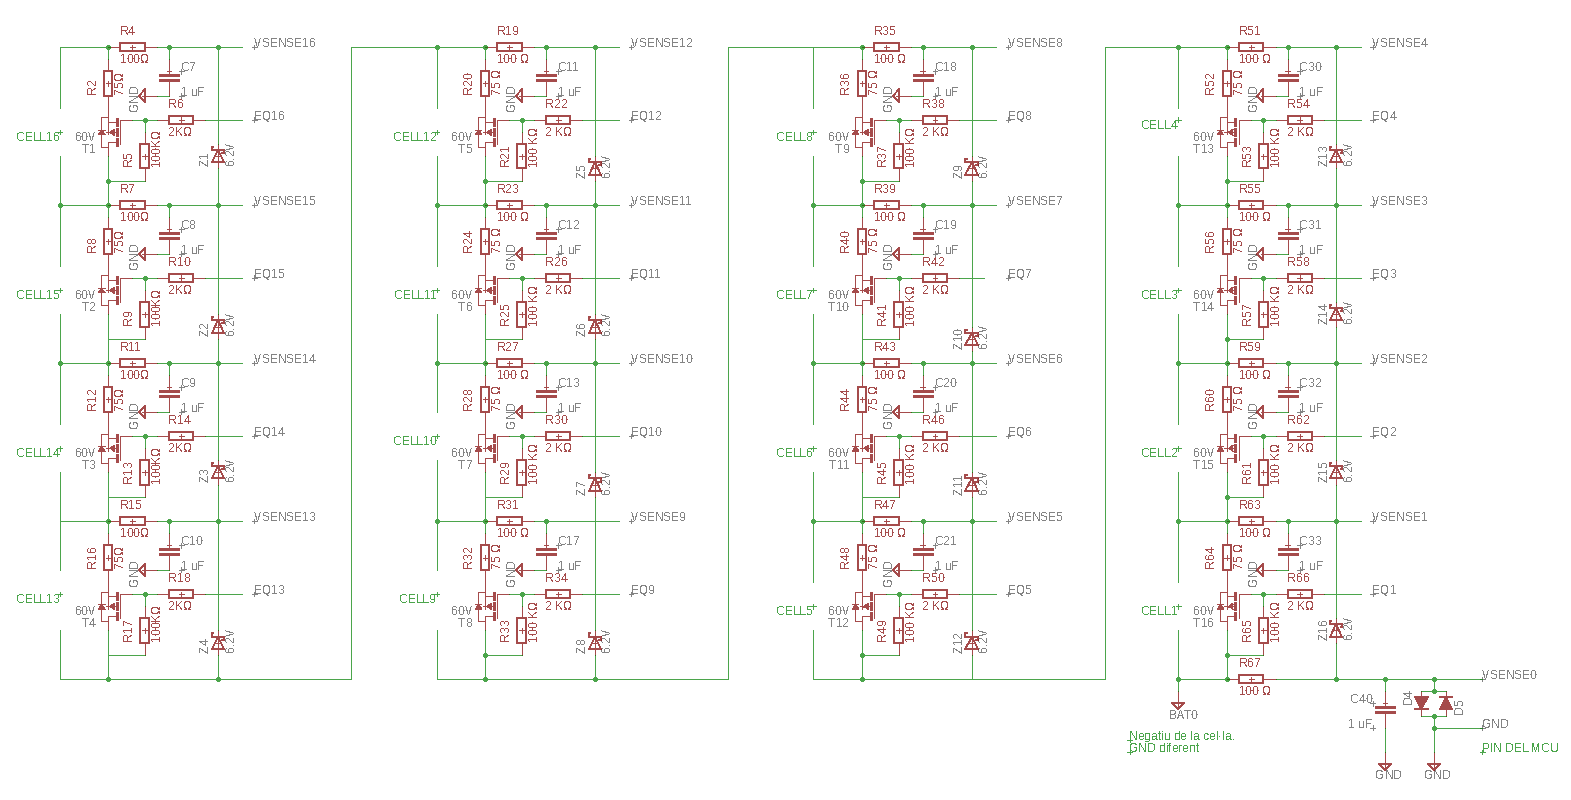
\includegraphics[width=\textwidth, height=10cm] {Prototip/schbalancing.png}
    \caption{Circuit de balanceig de les cel·les}
\end{figure}

\subsection{Tractament de la temperatura}
Encara que l'integrat de per sí ja porta sensors de temperatura interns, el fet de disposar d'entrades analògiques per a mesurar el voltatge ha fet que no les puguem deixar passar. La temperatura es calcula amb un termistor, que és una resistència variable la qual varia en funció de la temperatura. La temperatura és mesurada de forma diferencial per parelles. Fins a 4 mòduls de temperatura poden estar connectats a l'integrat, ja que l'integrat disposa de 8 entrades analògiques, les quals van per parelles. Aquestes entrades són gestionades per l'integrat, però en cap moment en processen la seva informació, solament envien la informació al micro el qual serà l'encarregat de processar aquestes temperatures.

A més el senyal és filtrat mitjançant un filtre RC per a que el senyal entri lo més net possible i no provoqui alteracions, encara que amb la mesura diferencial ja es tenen en compte.

\begin{figure}[H]
	\centering
    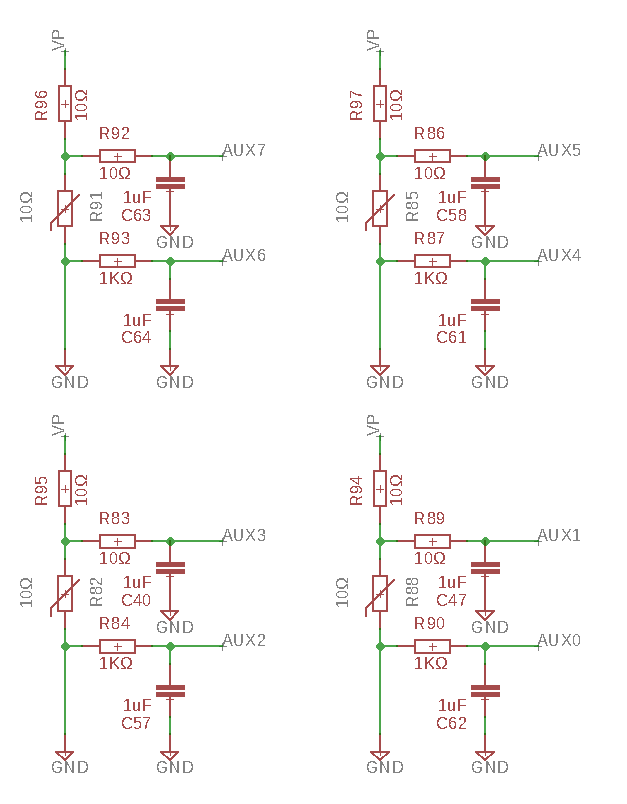
\includegraphics[width=\textwidth, height=14cm] {Prototip/schtemperatura.png}
    \caption{Mesurament extern de la temperatura.}
\end{figure}


\subsection{Comunicació entre Mestre/Esclau}

Depenent de si estem parlant d'un mòdul mestre o un mòdul esclau, aquest esquemàtic pot variar. En el cas de que sigui la placa mestre, les connexions cap a un mòdul n-1 no tenen cap mena de sentit ja que la placa mestre és la placa 1. Això vol dir que només necessita de la part de l'esquemàtic que es connecta a la següent placa BMS.

\begin{figure}[H]
	\centering
    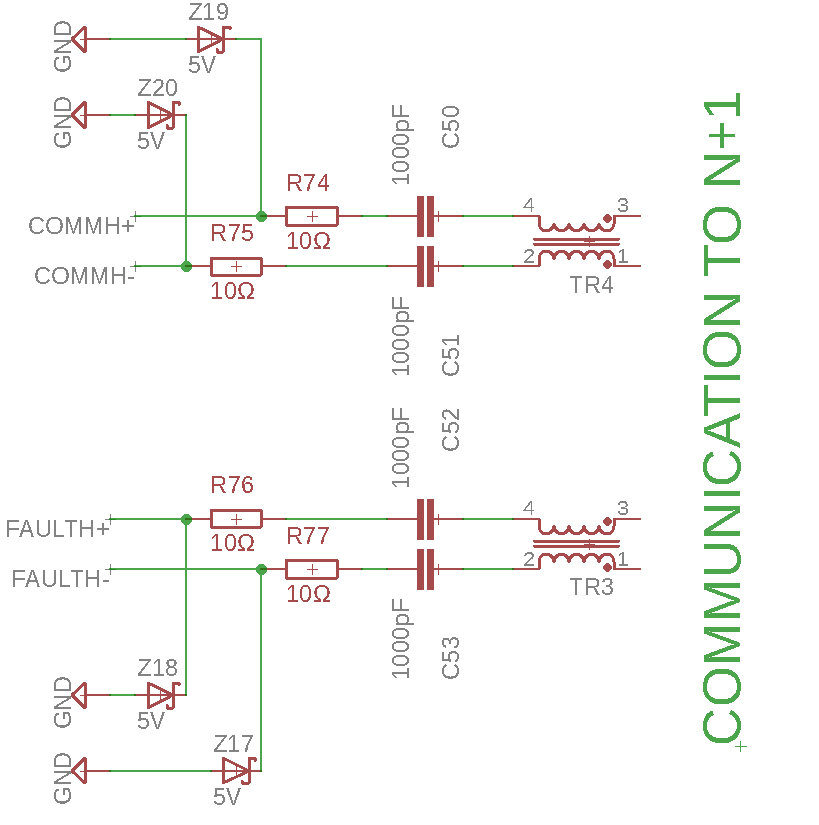
\includegraphics[width=\textwidth, height=12cm] {Prototip/schcomm+1.png}
    \caption{Comunicació amb el mòdul BQ76pl455a-q1 n+1.}
\end{figure}

\newpage

En canvi si estem parlant d'un mòdul esclau, aquest pot tenir els dos esquemàtics, és a dir, que ha de poder comunicar-se amb el mòdul inferior a ell i el mòdul superior a ell. Quan s'arriba a l'últim mòdul aquest només té l'esquemàtic per parlar amb el mòdul anterior. 

\begin{figure}[H]
	\centering
    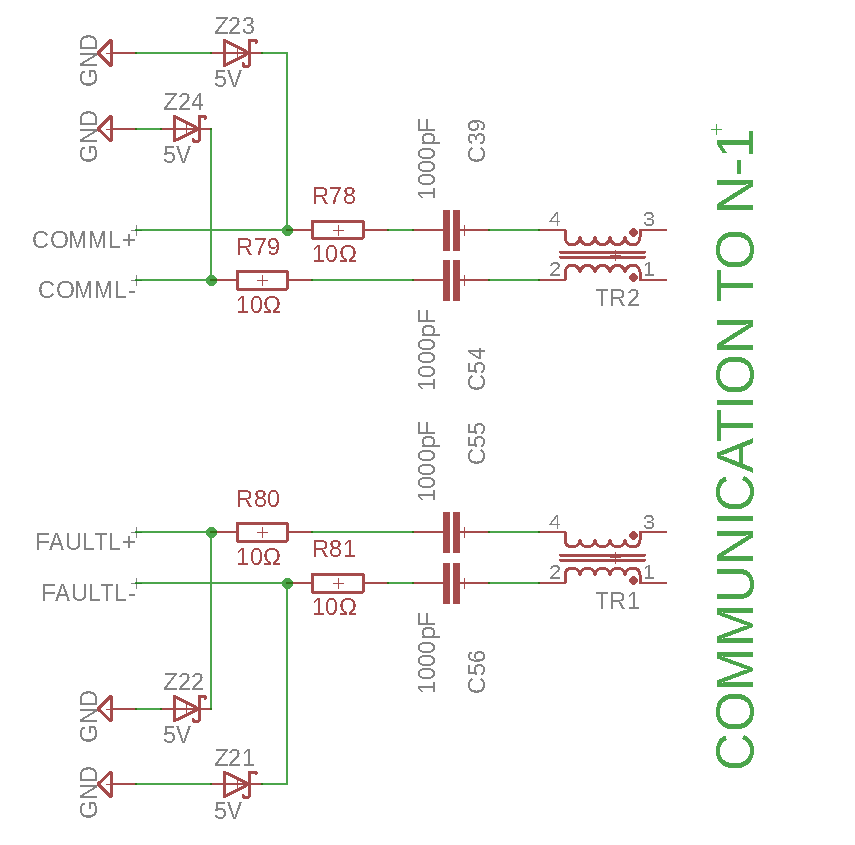
\includegraphics[width=\textwidth, height=14cm] {Prototip/schcomm-1.png}
    \caption{Comunicació amb el mòdul BQ76pl466a-q1 n-1.}
\end{figure}

\newpage 

La implementació d'ambdós esquemàtics és exactament la mateixa, amb la diferència de que estan connectats a diferents pins, ja que per comunicar-se amb el mòdul superior es parla a través dels pins acabats en H i per comunicar-se amb els inferiors amb els pins acabats en L. 

El circuit disposa de díodes zener, els quals limiten a que tot el voltatge sobrant no circuli pel circuit i sigui el zener qui l'atrapi. Amb això aconseguim que el voltatge no pugui sortir dels rangs de funcionament de les comunicacions. A més per comunicar entre dispositius BMS, el sistema de comunicacions queda totalment aïllat per un transformador (trafo). Aquest s'encarrega d'aïllar aquest voltatge per tal de poder-ho connectar de forma ideal al següent o anterior mòdul.

\subsection{Integrat BQ76pl455a-q1}

En aquest apartat tractarem l'integrat com a tal, encara que no es vegi d'una forma clara, s'utilitzen tots els pins d'aquest microcontrolador, \newline únicament que la connexió no es visible. El que si que es pot apreciar d'aquesta figura és com es realitza la comunicació entre la part que gestiona les bateries i la part que realitza el càlcul mitjançant els pins OUT. A més a més es veu la implementació dels pins CHP/CHM que s'utilitzen per a l'AFE. No s'ha entrat en detall en aquests aspectes degut a que simplement s'han seguit les especificacions del fabricant.

Cal destacar també que el VIO disposa de dos condensadors a massa per a evitar canvis bruscs de voltatge en aquest pin. 

\begin{figure}[H]
	\centering
    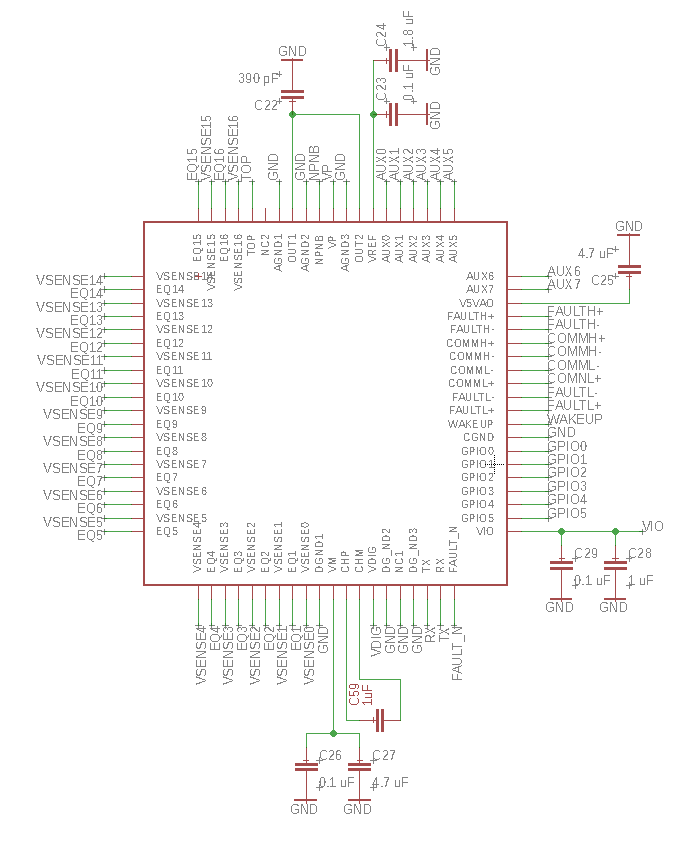
\includegraphics[width=\textwidth, height=15cm] {Prototip/schbq.png}
    \caption{Integrat BQ76pl455a-q1.}
\end{figure}

\newpage 

A més tampoc s'ha explicat res de les masses degut a que la implementació no ha pogut acabar de fer-se. El fabricant recomana l'utilització de diferents capes de massa a la PCB per tal d'evitar els retorns que els senyals analògics confronten amb els senyals digitals si van per la mateixa posició de la PCB. El fabricant mostra la següent figura indicant que cal realitzar aquesta diferenciació per tal de fer treballar el microcontrolador amb senyals el més nets possibles.

\begin{figure}[H]
	\centering
    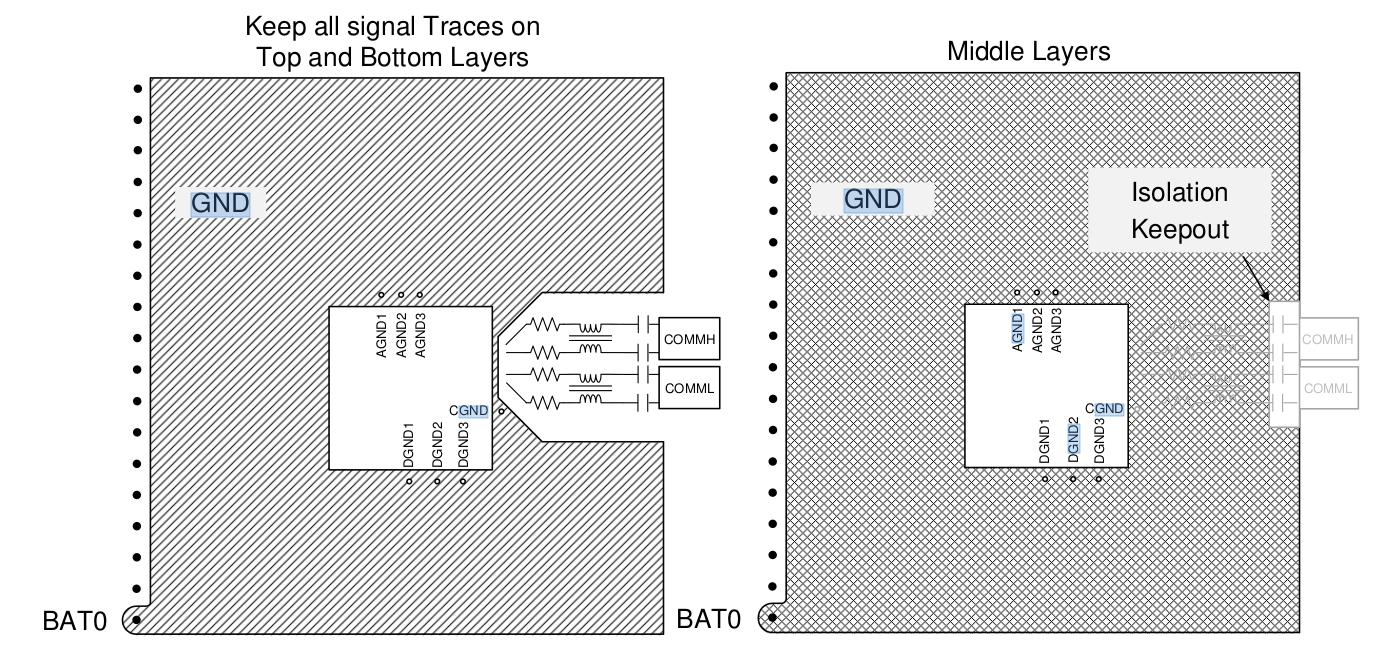
\includegraphics[width=\textwidth, height=7cm] {Prototip/pcbgnd.png}
    \caption{Capa de masses de la futura PCB.}
\end{figure}

\newpage 

\subsection{Microcontrolador Atmel}
L'esquemàtic del microcontrolador ha estat extret del propi disseny de l'Arduino Mega. S'ha aprofitat tot el sector del rellotge del microcontrolador, del regulador de voltatge, per a què al micro li arribi un senyal pur de 5V i la implementació del reset. A més, per a poder carregar el programa al microcontrolador és precís d'un protocol de comunicacions entre un ordinador i aquest microcontrolador. La solució que normalment empra Arduino és mitjançant l'ús d'una comunicació Serial a partir de l'USB. El problema que té aquest tipus de comunicació és que requereix d'una electrònica molt més elaborada afegint un segon integrat (Atmega16U2), el qual permet gestionar el senyal provinent del Serial. És per això que la injecció de codi en el nostre cas es dóna a través del protocol SPI. L'integrat Atmega2560 permet el reconeixement d'aquest protocol de forma directa, amb la qual cosa només afegint un header per a poder connectar-nos nosaltres és suficient per a la injecció de codi.

El serial que s'utilitza per comunicar-nos entre el microcontrolador i el BQ és el Serial3, per el seu alt rendiment i configurabilitat. Els pins de GPIO es connecten al port A complert i els pins de WAKEUP i FAULTN es connecten als pins lliures del port B, que és el port més precís de l'Atmega2560.
\begin{figure}[H]
	\centering
    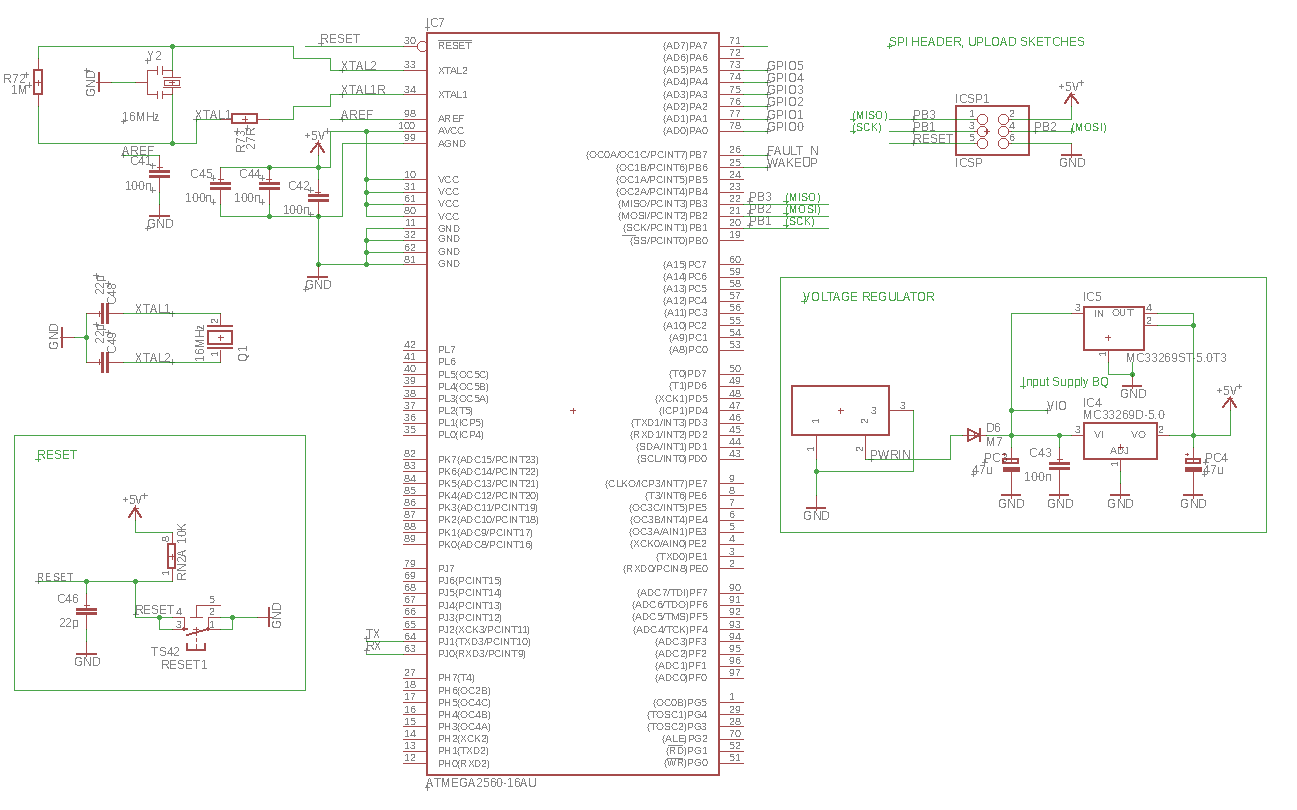
\includegraphics[width=\textwidth, height=10cm] {Prototip/schatmega2560.png}
    \caption{Implementació de l'Atmega 2560.}
\end{figure}